% SC2005 Ch07 — Virtual Memory (no \documentclass)
\chapter{Virtual Memory}
\label{ch:vmem}

\begin{quote}
\emph{Virtual memory lets a process believe it owns a large, contiguous
address space backed by disk.} This chapter explains demand paging, replacement,
and thrashing.
\end{quote}

\noindent\textbf{Learning Outcomes.} After this chapter you will be able to:
\begin{enumerate}[label=(L\arabic*)]
  \item explain demand paging, page faults, and effective access time;
  \item simulate FIFO, Optimal, LRU, and Clock page replacement;
  \item define working set, thrashing, and frame allocation;
  \item reason about copy-on-write, memory-mapped files, and swapping;
  \item evaluate VM performance via fault rate and locality.
\end{enumerate}

% ============================================================
\section{Demand Paging}
\label{sec:demand-paging}

In \emph{demand paging}, pages are loaded only when accessed. A page table
entry has a \emph{valid} bit (in memory), \emph{dirty} bit, and reference bit.
On access to an invalid page, a \emph{page fault} traps to the kernel, which
finds a free frame (or evicts one), reads the page from disk, updates the
table, and restarts the faulting instruction.

\begin{figure}[h!]
\centering
\begin{tikzpicture}[scale=0.74, every node/.style={font=\scriptsize},
  s/.style={draw, rounded corners, align=center, minimum width=2.6cm, minimum height=0.7cm}]
  \node[s, fill=blue!12] (a) at (0,1.8) {Access virtual page};
  \node[s, fill=orange!15] (b) at (3.6,1.8) {TLB / page table\\ valid?};
  \node[s, fill=green!14] (c) at (3.6,0.4) {Translate\\ + access RAM};
  \node[s, fill=red!14] (d) at (0,0.4) {Page fault:\\ trap to kernel};
  \node[s, fill=violet!12] (e) at (0,-0.9) {Load from disk\\ + update table};
  \draw[-{Stealth}, thick, blue!60!black] (a)--(b);
  \draw[-{Stealth}, thick, green!50!black] (b)--(c) node[midway,above,font=\tiny]{yes};
  \draw[-{Stealth}, thick, red!60!black] (b)--(d) node[midway,left,font=\tiny]{no};
  \draw[-{Stealth}, thick, red!60!black] (d)--(e);
  \draw[-{Stealth}, thick, dashed, green!50!black] (e) -- ++(2.0,0) |- (b);
\end{tikzpicture}
\caption{Demand paging flow: fast path vs.\ page-fault path.}
\label{fig:demand-paging}
\end{figure}

Effective access time with fault rate $p$ and fault service time $t_f$:
\[
  t_{\text{eff}} = (1-p)\,t_{\text{mem}} + p\,t_f,
  \qquad t_f \approx 8\text{--}20\text{\,ms (disk I/O)}.
\]
Even $p=0.001$ with $t_f=10$\,ms and $t_{\text{mem}}=100$\,ns gives
$t_{\text{eff}}\approx 10\mu$s --- $100\times$ slower. Locality and good
replacement keep $p$ tiny.

\begin{example}[Effective access time]
If $p=10^{-4}$, $t_{\text{mem}}=100$\,ns, $t_f=8$\,ms:
$t_{\text{eff}}=0.9999\cdot100\text{ns}+10^{-4}\cdot8\text{ms}\approx 900$\,ns
--- almost $10\times$ slower than no faults. Keeping $p<10^{-5}$ is essential.
\end{example}

\subsection{Copy-on-Write and Memory-Mapped Files}
\texttt{fork} shares pages read-only; a write fault copies the page.
\texttt{mmap} maps files directly into the address space, with demand paging
handling I/O --- the basis for shared libraries and fast file access.

% ============================================================
\section{Page Replacement}
\label{sec:replacement}

When no free frame exists, the OS must evict a page. Goals: minimize future
faults, avoid Belady's anomaly (more frames $\to$ more faults, as in FIFO).

\begin{itemize}
  \item \textbf{FIFO:} evict oldest page --- simple, suffers Belady's anomaly.
  \item \textbf{Optimal (OPT):} evict page whose next use is farthest --- optimal
        but requires future knowledge; used as benchmark.
  \item \textbf{LRU:} evict least recently used --- exploits temporal locality;
        implement via counters, stack, or reference bits.
  \item \textbf{Clock (second-chance):} circular list with reference bits;
        on fault, sweep: clear $R=1$ and advance, evict first $R=0$ page.
\end{itemize}

\begin{figure}[h!]
\centering
\begin{tikzpicture}[scale=0.74, every node/.style={font=\scriptsize},
  b/.style={draw, minimum width=1.1cm, minimum height=0.6cm, align=center}]
  \node[font=\footnotesize\bfseries] at (-1.2,1.2) {Clock:};
  % circular frames
  \foreach \i/\lbl in {0/A,1/B,2/C,3/D} {
    \node[b, fill=blue!12] (f\i) at (\i*1.6,0.4) {$\lbl$\strut\\ \tiny $R{=}0/1$};
  }
  \draw[-{Stealth}, thick, red!60!black] (1.2,-0.3) -- (1.8,-0.3) node[midway,below,font=\tiny]{hand};
  \draw[->, thick, green!50!black] (5.4,0.4) arc (0:300:0.5);
  \node[font=\tiny, align=left] at (6.8,0.4) {Sweep:\\if $R{=}1$ clear\\else evict};
  \node[font=\tiny] at (0.8,1.35) {Reference bits on access};
\end{tikzpicture}
\caption{Clock (second-chance) replacement: circular sweep over reference bits.}
\label{fig:clock}
\end{figure}

\begin{figure}[h!]
\centering
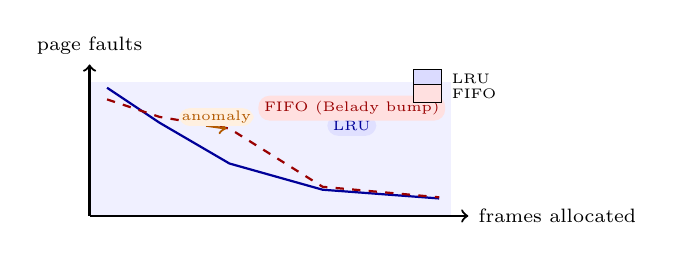
\begin{tikzpicture}[scale=0.74, every node/.style={font=\scriptsize}]
  \fill[blue!6] (0,0) rectangle (6.2,2.3);
  \draw[->, thick] (0,0) -- (6.5,0) node[right]{frames allocated};
  \draw[->, thick] (0,0) -- (0,2.6) node[above]{page faults};
  \draw[thick, blue!60!black] (0.3,2.2) -- (1.2,1.6) -- (2.4,0.9) -- (4.0,0.45) -- (6.0,0.3);
  \draw[thick, red!60!black, dashed] (0.3,2.0) -- (1.2,1.7) -- (2.4,1.5) -- (4.0,0.5) -- (6.0,0.32);
  \node[font=\tiny, fill=blue!12, rounded corners, inner sep=2pt, text=blue!60!black] at (4.5,1.55) {LRU};
  \node[font=\tiny, fill=red!12, rounded corners, inner sep=2pt, text=red!60!black] at (4.5,1.85) {FIFO (Belady bump)};
  \draw[->, thick, orange!70!black] (2.0,1.55) -- (2.35,1.5) node[midway,above,font=\tiny, fill=orange!12, rounded corners, inner sep=1pt]{anomaly};
  \node[draw, fill=blue!14, minimum width=0.35cm, minimum height=0.14cm] at (5.8,2.35) {}; \node[font=\tiny, anchor=west] at (6.05,2.35) {LRU};
  \node[draw, fill=red!12, minimum width=0.35cm, minimum height=0.14cm] at (5.8,2.10) {}; \node[font=\tiny, anchor=west] at (6.05,2.10) {FIFO};
\end{tikzpicture}
\caption{Page faults vs.\ frames: LRU monotonic; FIFO can exhibit Belady's anomaly.}
\label{fig:belady}
\end{figure}

\begin{remark}[Belady's anomaly intuition]
FIFO evicts by age, not recency. A longer queue can retain ``old but hot''
pages while evicting recently used ones that FIFO happened to admit later.
Stack algorithms (LRU, OPT) never suffer this because their resident sets are
nested: $M(k)\subseteq M(k+1)$.
\end{remark}

\begin{example}[Reference string: 1,2,3,4,1,2,5 -- 3 frames]
FIFO faults on 1,2,3,4,5 (7 faults with Belady cases); LRU faults on
1,2,3,4,5 (similar here but better on locality-heavy strings); Clock
approximates LRU with one reference bit per page.
\end{example}

% ============================================================
\section{Thrashing and Frame Allocation}
\label{sec:thrashing}

\emph{Thrashing} occurs when the system spends more time paging than executing,
typically when total working sets exceed available frames. The \emph{working set}
$W(t,\Delta)$ is the set of pages referenced in the last $\Delta$ accesses;
allocating fewer frames than $|W|$ guarantees high fault rates.

Cures: working-set model (ensure each process keeps its $W$ resident),
page-fault frequency control, and simply admitting fewer processes
(\emph{load control}). Global replacement can let one process thrash others;
local (per-process) replacement isolates faults.

\begin{lstlisting}[language=C,caption={Simulating LRU faults}]
#include <stdio.h>
#define FRAMES 3
int lru_faults(int *ref, int n){
    int frame[FRAMES], last[FRAMES], t=0, faults=0;
    for(int i=0;i<FRAMES;i++) frame[i]=-1, last[i]=-1;
    for(int k=0;k<n;k++){ int p=ref[k], hit=0;
        for(int i=0;i<FRAMES;i++) if(frame[i]==p){ hit=1; last[i]=t++; break; }
        if(!hit){ faults++; int v=0; // evict LRU
            for(int i=1;i<FRAMES;i++) if(last[i]<last[v]) v=i;
            frame[v]=p; last[v]=t++;
        }
    } return faults;
}
\end{lstlisting}

% ============================================================
\subsection{Frame Allocation and Locality}
Allocate too few frames and the process faults constantly; too many and CPU
utilization drops (fewer processes fit). The working-set window $\Delta$
should span a locality phase; sampling reference bits periodically estimates it.
Thrashing is visible as high paging I/O with low CPU use --- the system
pages furiously but makes no progress.

% prepaging trades I/O for reduced fault latency
% effective only with good locality prediction
\begin{remark}[Prepaging]
\emph{Prepaging} (prefetching pages before they fault) helps when locality is
predictable (sequential file access). Mispredicted prepaging wastes I/O and
frames, so most systems use demand paging with limited speculative read-ahead.
\end{remark}

\section{Exercises}
\label{sec:ch07-ex}
\begin{exercise}
Given $t_{\text{mem}}=100$\,ns, $t_f=10$\,ms, what fault rate keeps
$t_{\text{eff}}<200$\,ns?
\end{exercise}
\begin{exercise}
Simulate FIFO, LRU, and Clock on reference string
$1,2,3,4,1,2,5,1,2,3,4,5$ with 3 and 4 frames. Identify any Belady anomaly.
\end{exercise}
\begin{exercise}
Explain why LRU is a stack algorithm (more frames cannot increase faults) while
FIFO is not. Give a concrete Belady example.
\end{exercise}
\begin{exercise}
Define working set $W(t,\Delta)$. How does $\Delta$ affect thrashing detection?
What happens if $\Delta$ is too small or too large?
\end{exercise}
\begin{exercise}
Describe copy-on-write for \texttt{fork} in terms of page-table bits and fault
handling. When is the copy actually performed?
\end{exercise}
